\documentclass[main.tex]{subfiles}
\begin{document}
\section{Theoretische Grundlagen}

In diesem Abschnitt werden die theoretischen Grundlagen, die diese Arbeit
benötigt, erläutert.

\subsection{Heisenberg Modell}

Um das System von mehreren magnetischen Momenten zu beschreiben, wird das
klassische Heisenberg Modell verwendet. Es beschreibt die Wechselwirkung
zwischen den magnetischen Momenten der einzelnen Atome.

Die magnetischen Momente \(\vec{\mu}\) werden als Vektoren der Länge
\(\mu_{\text{S}}\) angenommen.
Die normierten und dimensionslosen magnetischen Momente werden mit \(\vec{S}\)
bezeichnet:

\begin{align}
	\vec{S} = \frac{\vec{\mu}}{\mu_{\text{S}}}
\end{align}

Da ein Antiferromagnet betrachtet wird, bei dem die magnetischen Momente in
entgegengesetzte Richtungen zeigen und die Beträge der magnetischen Momente
gleich sind gilt zusätzlich \(\mu_{\text{S},i} = \mu_{\text{S},j} = \mu_{S}\).

Diese Wechselwirkungen werden durch die Hamilton Funktion beschrieben, welche
sich aus mehreren Komponenten zusammensetzt:
\todo{Einzelne komponenten stärker ausführen?}

\subsubsection*{Heisenberg Austauschwechselwirkung}
% Heisenberg Austauschwechselwirkung

Die Heisenberg Austauschwechselwirkung beschreibt die Wechselwirkung zwischen
den magnetischen Momenten der einzelnen Atome aufgrund von überlappten
Wellenfunktionen~\cite{Heisenberg-Ferromagnetismus}. Sie ist die dominierende
Wechselwirkung in Antiferromagneten. Klassisch ist sie proportional zum
Skalarprodukt der magnetischen Momente:

\begin{align}
	\mathcal{H}_{\text{EXC}} = -\sum_{i,j} J_{ij} \vec{S}_i \cdot \vec{S}_j\label{eq:hamilton-heisenberg-exc}
\end{align}

\subsubsection*{Dzyaloshinskii-Moriya Wechselwirkung}
% Dzyaloshinskii-Moriya interaction 

Die Dzyaloshinskii-Moriya Wechselwirkung (DMI) beschreibt die indirekte
antisymmetrische Interaktion von zwei Spins\cite{DMI}. Sie ist in
Antiferromagneten die zweitstärkste Wechselwirkung und ist proportional zum
Kreuzprodukt der magnetischen Momente:

\begin{align}
	\mathcal{H}_{\text{DMI}} = \sum_{i,j} \vec{D}_{ij} \cdot (\vec{S}_i
	\times
	\vec{S}_j)\label{eq:hamilton-dmi}
\end{align}

\subsubsection*{Magnetische Anisotropien}
Magnetische Momente können eine Präferenz für eine bestimmte Richtung haben.
Die Energie, die aufgewendet werden muss, um das magnetische Moment aus dieser
Richtung zu drehen, wird als Anisotropie bezeichnet. Es gibt verschiedene Arten
von Anisotropien:\\

% \subsubsubsection{Uniaxiale Anisotropie}
Viele Materialien sind in einer Richtung Isotrop, d.h. die Anisotropie ist in
dieser Richtung Null. In den anderen Richtungen ist die Anisotropie uniaxial,
d.h. die Anisotropie ist in diesen Richtungen gleich. Die uniaxiale Anisotropie
kann durch die Kristallstruktur des Materials oder durch die Dipol-Dipol
Wechselwirkung entstehen.\\

\begin{align}
	\mathcal{H}_{\text{2A}} = -\sum_{i} \qty(\vec{S}_i)^\dagger
	\mathbf{d}_i
	\vec{S}_i\label{eq:hamilton-2a}
\end{align}

% \subsubsubsection{Anisotropie aus der Kristallstruktur} 
% alternativ: Anisotropie der Kristallfelder
\todo{erklärung Kubische Anisotropie bzw. 4. Ordnung Anisotropie}
% Kubische Anisotropie
\begin{align}
	\mathcal{H}_{\text{4A}} = -\sum_{i} L_{i,x} \qty(\vec{S}_{i,y})^2
	\qty(\vec{S}_{i,z})^2 - L_{i,y} \qty(\vec{S}_{i,z})^2
	\qty(\vec{S}_{i,x})^2
	-
	L_{i,z} \qty(\vec{S}_{i,x})^2 \qty(\vec{S}_{i,y})^2\label{eq:hamilton-4a}
\end{align}\cite{GrossMarx}

% \subsubsubsection{Zwei-Ionen Anisotropie}
\todo{erklärung zwei-Ionen Anisotropie}

\begin{align}
	\mathcal{H}_{\text{TIA}} = -\sum_{i,j} \vec{S}_i \mathbf{\kappa}_{ij}
	\vec{S}_j\label{eq:hamilton-tia}
\end{align}
\subsubsection*{Zeeman Wechselwirkung}
% Zeeman
Bei einem äußeren Magnetfeld \(B_\text{ext}\) wirkt auf jedes magnetische
Moment auch noch die Zeeman Wechselwirkung:

\begin{align}
	\mathcal{H}_{\text{Z}} = - B_\text{ext} \sum_{i} \vec{\mu}_i = -
	B_\text{ext} \sum_{i} \mu_{\text{S},i} \cdot \vec{S}_i\label{eq:hamilton-zeeman}
\end{align}

% Dipol Dipol wechselwirkung
\subsubsection*{Dipol-Dipol Wechselwirkung}

Jedes magnetische Moment erzeugt ein Magnetfeld, welches aus hinreichender
Entfernung stehts wie ein Dipolfeld aussieht:

\begin{align}
	\vec{B}(\vec{r}) & = \frac{\mu_0}{4\pi} \qty[3 \frac{\vec{r}(\vec{\mu}
			\cdot
			\vec{r})}{r^5} -
		\frac{\vec{\mu}}{r^3}]\label{eq:dipolmoment}
\end{align}\cite{Nolting-3-elektrodynamik}

Wenn zwei magnetische Momente \(\vec{\mu}_i\) und \(\vec{\mu}_j\) in einem
Abstand \(r_{ij}\) zueinander stehen, wirkt auf das magnetische Moment
\(\vec{\mu}_i\) das Magnetfeld \(\vec{B}_j\) und auf das magnetische Moment
\(\vec{\mu}_j\) das Magnetfeld \(\vec{B}_i\). Die Wechselwirkungsenergie
zwischen den beiden magnetischen Momenten ist die Energie, die aufgewendet
werden muss, um die beiden magnetischen Momente aus dem Magnetfeld des jeweils
anderen zu entfernen. Die Wechselwirkungsenergie ist also proportional zum
Skalarprodukt der beiden Magnetfelder:

\begin{align}
	\mathcal{H}_{\text{DD}} & = \sum_{\substack{i,j           \\ i \neq j}}
	\frac{\mu_0}{4\pi}
	\cdot  \frac{3(\vec{\mu}_i \cdot \vec{r}_{ij})(\vec{\mu}_j \cdot
		\vec{r}_{ij})
	- \vec{\mu}_i \cdot \vec{\mu}_j \cdot r_{ij}^2}{r_{ij}^5} \\
	                        & = \sum_{\substack{i,j           \\ i \neq j}}
	\frac{\mu_0 \cdot \mu_{\text{S,i}} \cdot \mu_{\text{S,j}}}{4\pi}
	\cdot \frac{3(\vec{S}_i \cdot \vec{r}_{ij})(\vec{S}_j \cdot
		\vec{r}_{ij})
		- \vec{S}_i \cdot \vec{S}_j \cdot r_{ij}^2}{r_{ij}^5}\label{eq:hamilton-dd}
\end{align}

\subsection{Bewegungsgleichung: Landau-Lifschitz-Gilbert Gleichung}
% Landau-Lifschitz Gleichung (1935)
Um die Bewegung der magnetischen Momente zu beschreiben, muss aus der
Hamiltonfunktion die Bewegungsgleichung abgeleitet werden.
\todo{Herleitung über implizite Form}
Obwohl die Hamiltonfunktion klassisch ist, kann die Bewegungsgleichung über die
Quantenmechanik hergeleitet werden. Das Ehrenfest-Theorem besagt, dass die
zeitliche Änderung des Erwartungswertes eines Operators gleich dem
Erwartungswert des Kommutators des Operators mit der Hamiltonfunktion ist:

\begin{align}
	\dv{\hat{\vec{S}}_i}{t} = \frac{i}{\hbar} \expval{\qty[\hat{\vec{S}}_i,
			\hat{\mathcal{H}}]}
\end{align}%\cite{qm-1-Schwabl}

Mit der Relation \(\hat{\vec{S}}_i = \frac{\gamma_i}{\mu_{\text{S}}}
\hat{\vec{J}}_i\) und der Kommutatorrelation \(\qty[\hat{\vec{J}}_i,
	\hat{\vec{J}}_j] = i \hbar \cdot \varepsilon_{abc}
\hat{\vec{J}}_{c,i}\) (wobei
\(\varepsilon\) das Levi-Civita Symbol ist) ergibt sich:

\begin{align}
	\dv{\vec{S}_i}{t}                             & = -\frac{\gamma
	}{\mu_{\text{S}}}
	\qty(\vec{S}_i \times
	\vec{\mathcal{H}}_{\text{i}})
	\\
	\text{mit} \quad \vec{\mathcal{H}}_{\text{i}} & = -
	\pdv{\mathcal{H}}{\vec{S}_i}
\end{align}\cite{landau-lifshitz}

\todo{erklärung der einzelnen Terme}
% LL + Gilbert Gleichung (1955)
Diese Gleichung wurde 20 Jahre später von Gilbert um einen Dämpfungsterm
erweitert:

\begin{align}
	\dv{\vec{S}_i}{t} & = -\frac{\gamma }{\mu_{\text{S}}}\qty(\vec{S}_i
	\times
	\vec{\mathcal{H}}_{\text{i}}) + \alpha \qty(\vec{S}_i \times
	\dv{\vec{S}_i}{t})
\end{align}\cite{Gilbert-damping}

% gleichung in sich selbst einsetzen
\begin{align}
	\dv{\vec{S}_i}{t} & = -\frac{\gamma }{\mu_{\text{S}}}\qty(\vec{S}_i
	\times
	\vec{\mathcal{H}}_{\text{i}}) + \alpha \qty(\vec{S}_i \times
	\qty(-\frac{\gamma }{\mu_{\text{S}}}\qty(\vec{S}_i
		\times
		\vec{\mathcal{H}}_{\text{i}}) + \alpha \qty(\vec{S}_i \times
	\dv{\vec{S}_i}{t})))                                                \\
	                  & = -\frac{\gamma }{\mu_{\text{S}}}\qty(\vec{S}_i
	\times
	\vec{\mathcal{H}}_{\text{i}}) - \frac{\alpha\gamma}{\mu_\text{S}}
	\qty(\vec{S}_i \times \qty(\vec{S}_i \times
		\vec{\mathcal{H}}_{\text{i}})) +
	\alpha^2 \qty(\vec{S}_i \times \qty(\vec{S}_i \times
		\dv{\vec{S}_i}{t}))
\end{align}

\begin{align}
	\alpha^2 \qty(\vec{S}_i \times \qty(\vec{S}_i \times
	\dv{\vec{S}_i}{t})) & = -\alpha^2\dv{\vec{S}_i}{t}
\end{align}

\begin{align}
	\dv{\vec{S}_i}{t} & = -\frac{\gamma
	}{\mu_{\text{S}}(1+\alpha^2)}\qty[\qty(\vec{S}_i \times
		\vec{\mathcal{H}}_{\text{i}}) + \alpha \vec{S}_i \times
		\qty(\vec{S}_i \times
		\vec{\mathcal{H}}_{\text{i}})]
\end{align}

\todo{rauschen durch endliche Temperatur}

\begin{align}
	\vec{\mathcal{H}}_{\text{i}}                 & =
	-\pdv{\mathcal{H}}{\vec{S}_i} +
	\vec{\xi}_i(t)
	\\
	\expval{\vec{\xi}_i(t)}                      & = 0
	\\
	\expval{\xi_{i,\alpha}(t) \xi_{j,\beta}(t')} & = \frac{2\mu_\text{S}
		\alpha
	}{\gamma}k_\text{B} T \cdot \delta_{ij} \delta_{\alpha \beta}
	\delta(t-t')
\end{align}

\begin{figure}[H]
	\centering
	\subcaptionbox{\(T = \SI{0}{\kelvin} \)}
	{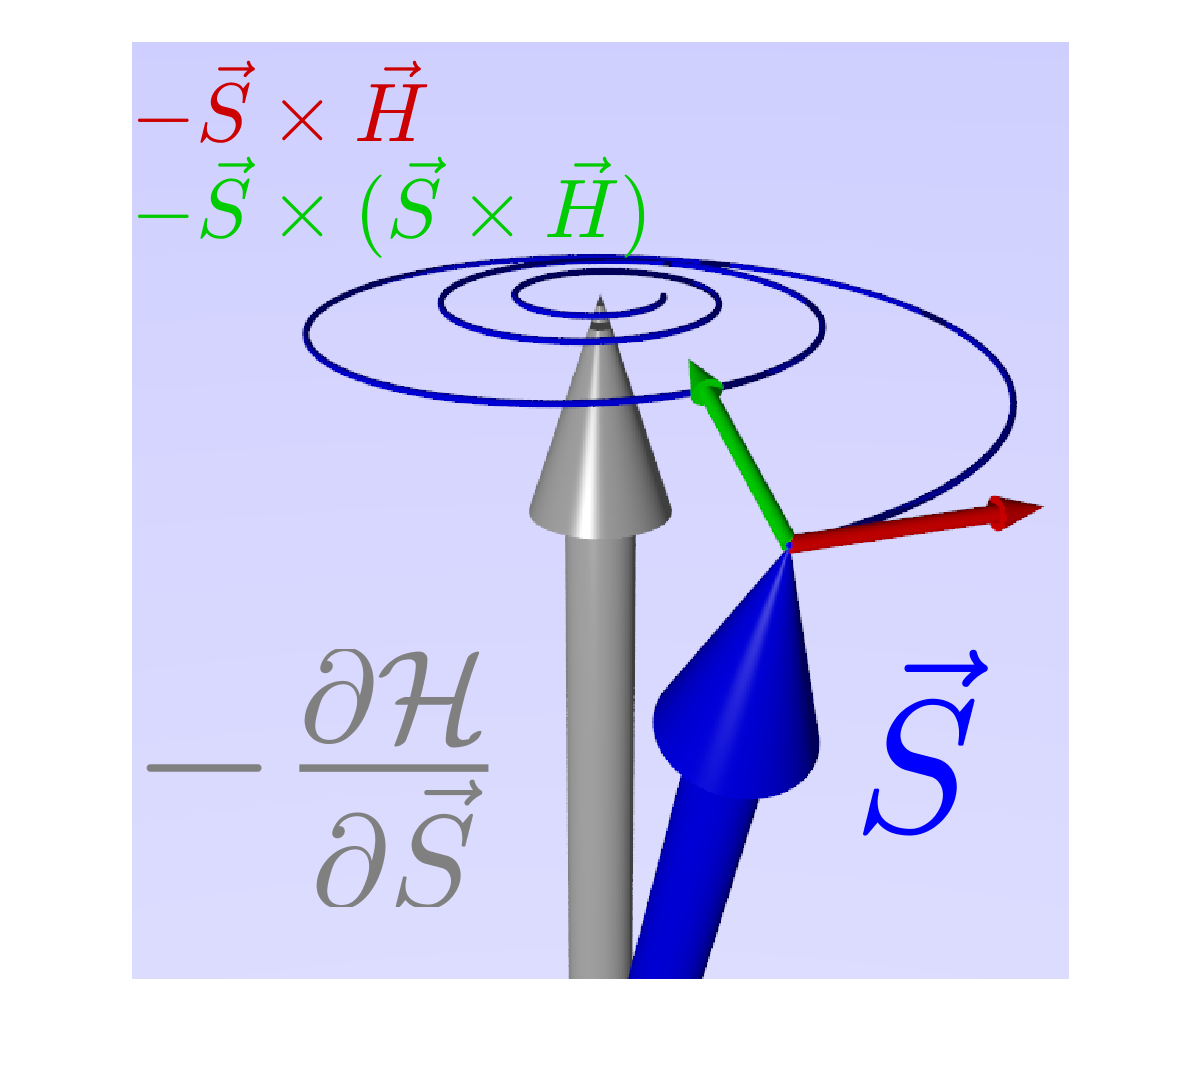
\includegraphics[width=0.45\textwidth]{bilder/jschlege/LLG_T0_labeled.png}}
	\subcaptionbox{\(T \gg \SI{0}{\kelvin} \)}
	{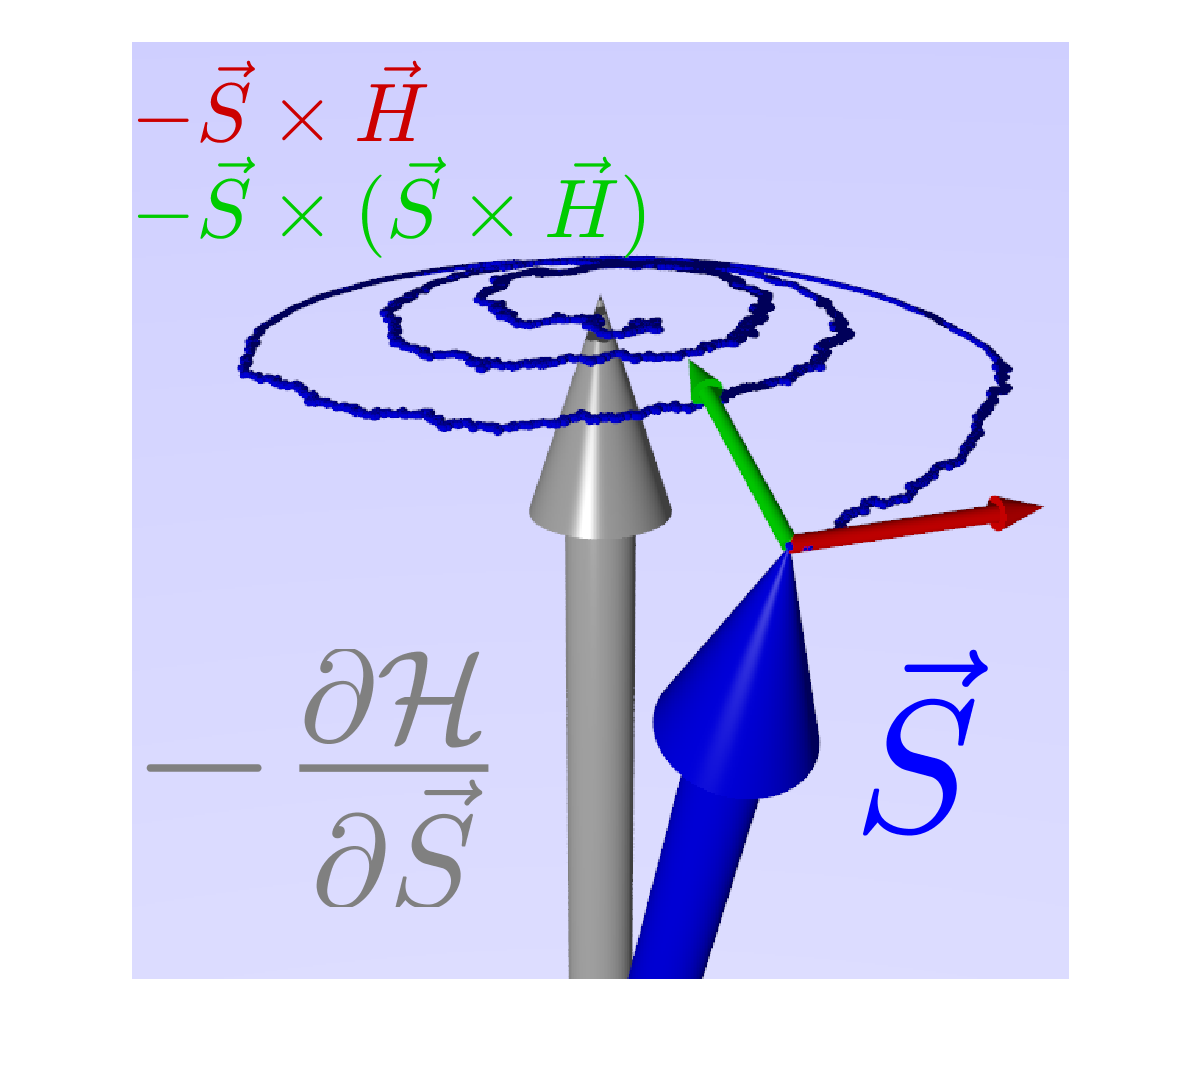
\includegraphics[width=0.45\textwidth]{bilder/jschlege/LLG_labeled.png}}
	\caption{Abhängig von der Simulationstemperatur ändert sich die Intensiät des Rauschens.\cite{schlegel-master}}
	\label{fig:llg-rauschen}
\end{figure}

\subsection{Modellierung von Orthoferrit}

Orthoferrite sind chemische Verbindungen der Form \ce{RFeO3}, wobei \ce{R} ein
Rest ist, durch den sich die verschiedenen Orthoferrite unterscheiden. Hier
bilden Samarium (\ce{Sm}) und Erbium (\ce{Er}) diese Restgruppe.

\begin{figure}[H]
	\centering

	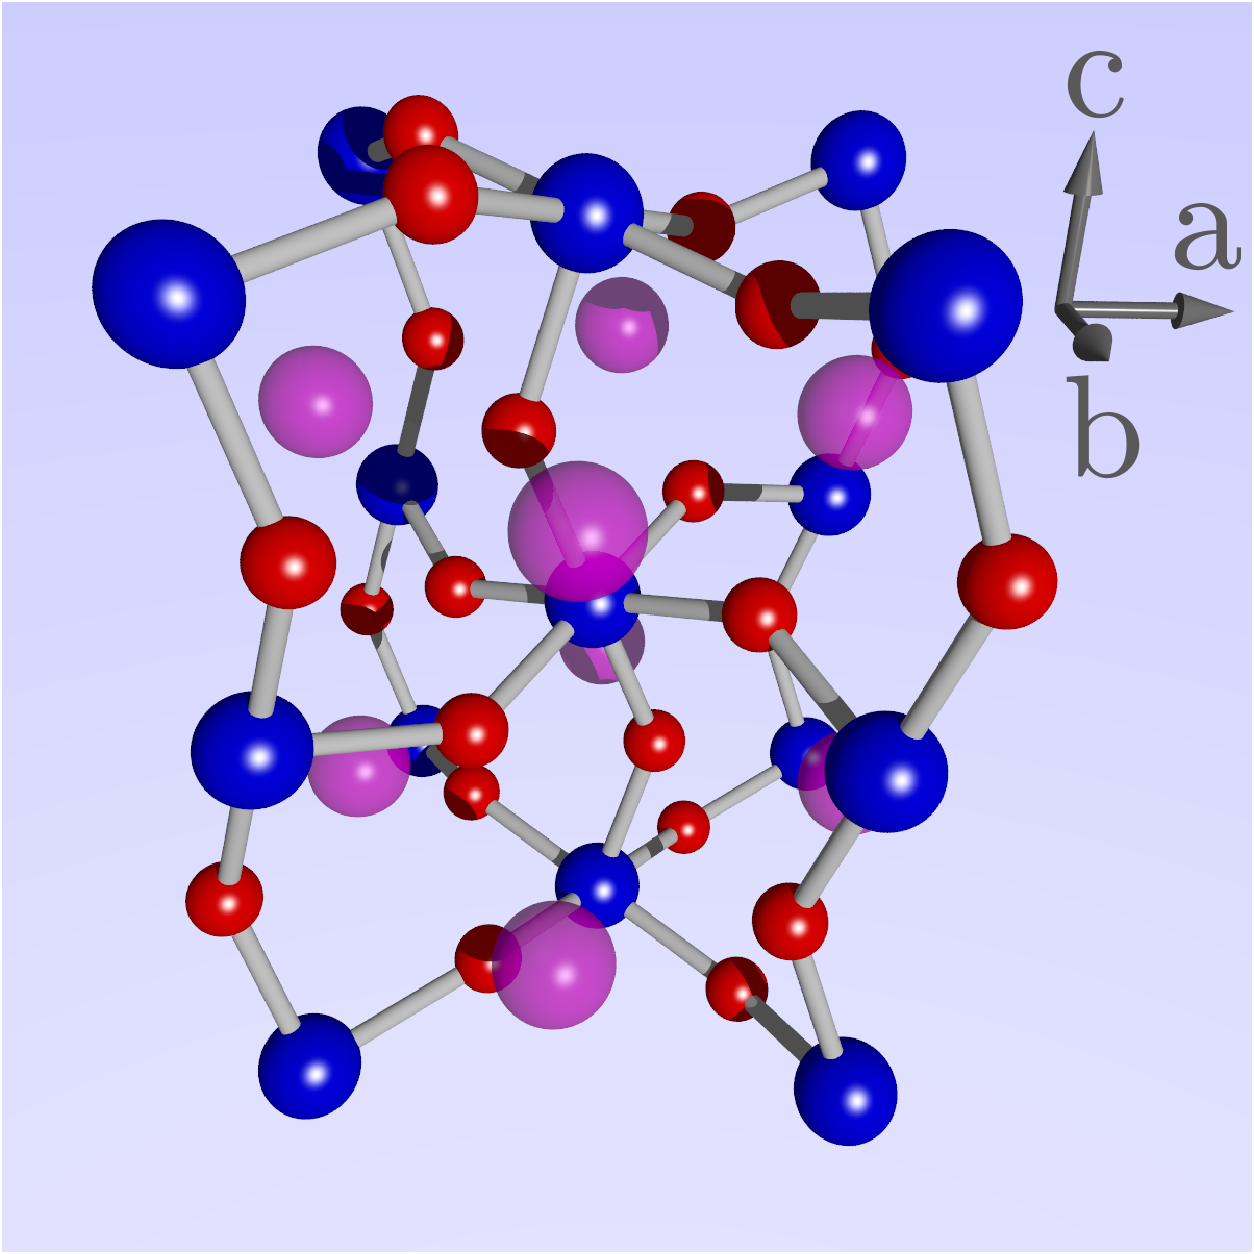
\includegraphics[width=0.4\textwidth]{bilder/jschlege/UnitCell_labeled.png}
	\caption{Kristallstruktur von
		\ce{ErFeO3}. Die Eisenatome sind dabei blau, die
		Sauerstoffatome rot und die Erbiumatome magenta gefärbt.
		\cite{schlegel-master}}
	\label{fig:orthoferrit}
\end{figure}

\begin{figure}[H]
	\centering
	\subcaptionbox{Einheitszelle mit DMI
		Vektoren(gelb)}
	{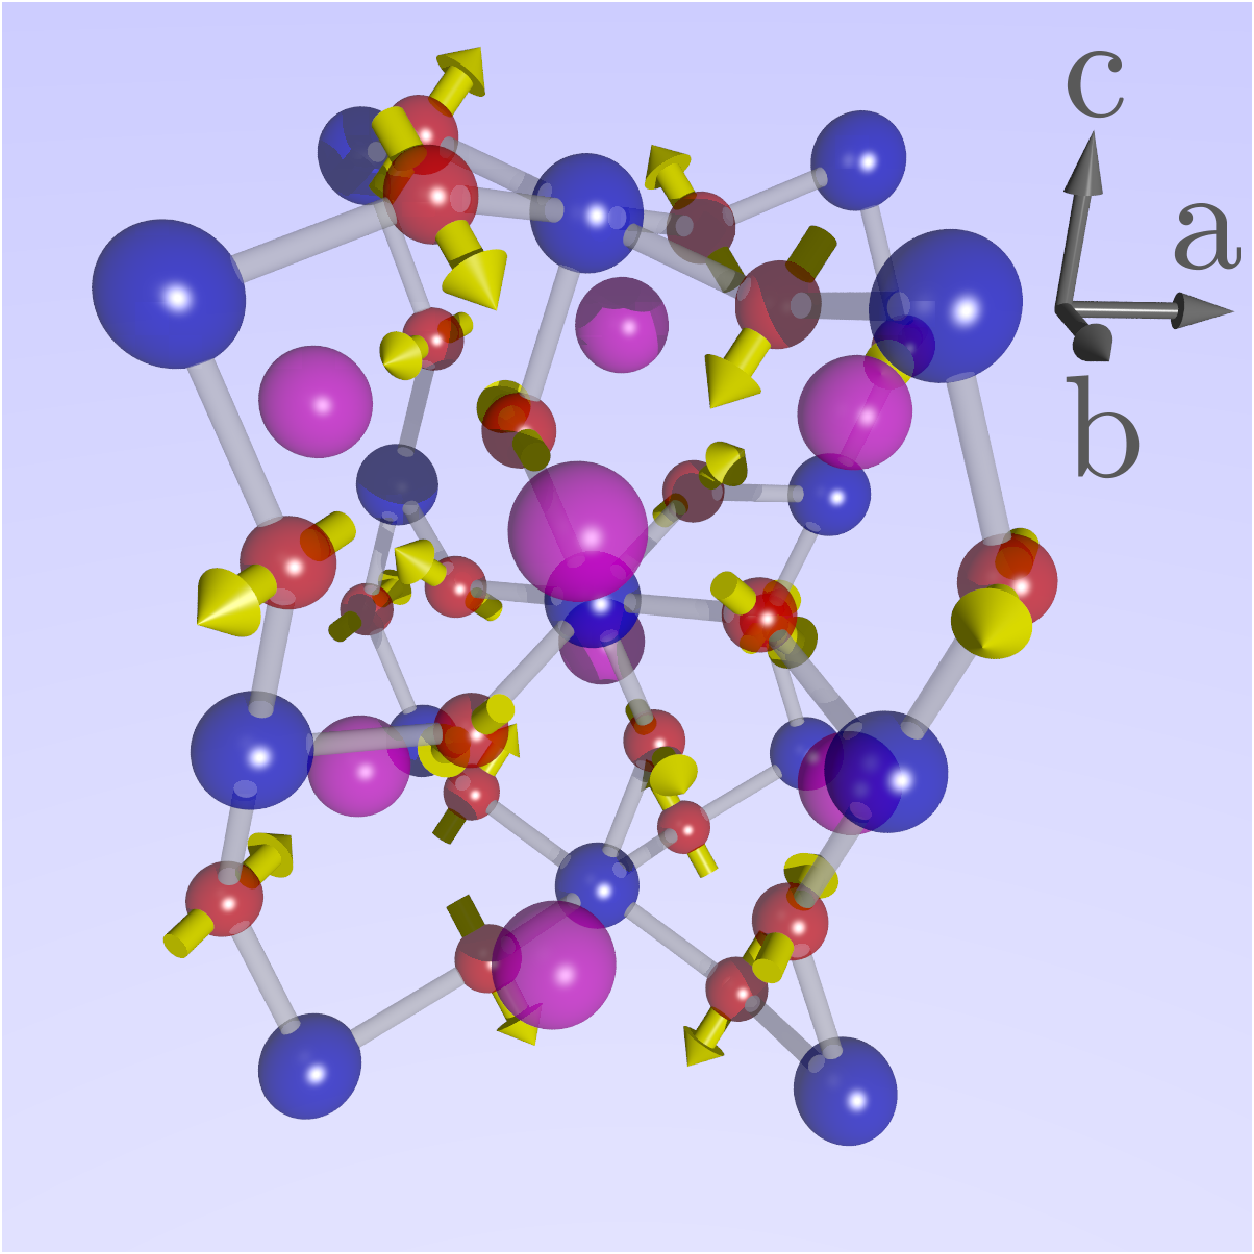
\includegraphics[width=0.3\textwidth]{bilder/jschlege/UnitCell_withDMI_labeled.png}}
	\subcaptionbox{Einheitszelle mit magnetischen Momenten (grün) für
		\(T<T_l\)}
	{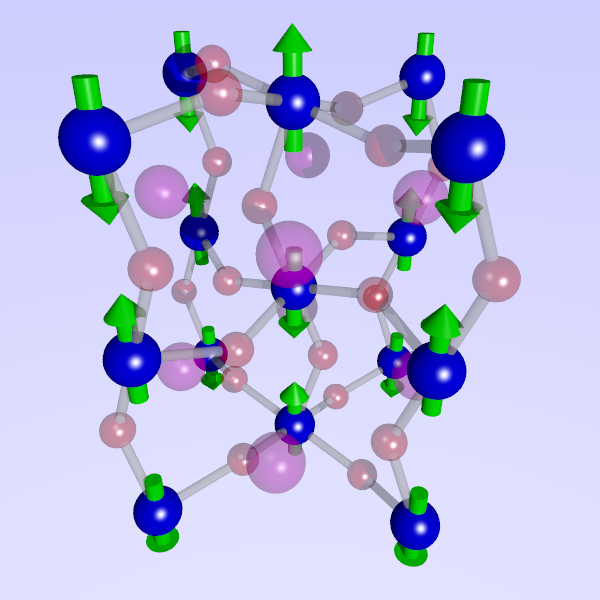
\includegraphics[width=0.3\textwidth]{bilder/jschlege/UnitCell_belowRT.png}}
	\subcaptionbox{Einheitszelle mit magnetischen Momenten (grün) für
		\(T>T_h\)}
	{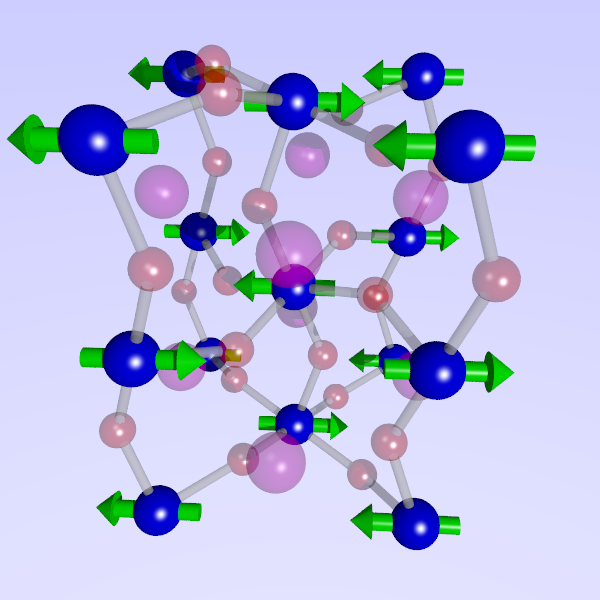
\includegraphics[width=0.3\textwidth]{bilder/jschlege/UnitCell_aboveRT.png}}
	\caption{\todo{ausführlichere} Kristallstruktur von \ce{ErFeO3}
		\cite{schlegel-master}}
	\label{fig:orthoferrit2}
\end{figure}

\todo{erklärung für Samarium (reorientierungstemperatur)}

Die Reorientierungstemperatur \(T_l < T < T_h\) liegt bei Erbiumferrit bei \todo{Wert einfügen}. Bei Samarium-Erbium-Ferrit (\ce{Sm_{0.7}Er_{0.3}FeO3}) liegt sie ungefähr bei Raumtemperatur, weshalb es im Experiment einfacher zu untersuchen ist.

% Parameter für Simulation
\todo{wer hat die Parameter bestimmt?}

Für die Simulation wird ein Modell von \ce{ErFeO3} verwendet, bei dem die Parameter \todo{welche explizit} angepasst wurden, um die Reorientierungstemperatur bei Raumtemperatur wie bei \ce{Sm_{0.7}Er_{0.3}FeO3} zu erhalten:

\begin{align}
	J_1             & = \SI{-22,32}{\milli\electronvolt}, \quad J_2 =
	\SI{-1,4}{\milli\electronvolt}
	\\
	\mathbf{d}      & = \mqty(
	\num{0.0153}    & \num{-0.0153}                                   & 0
	\\
	\num{-0.0153}   & \num{0.0153}                                    & 0
	\\
	0               & 0                                               &
	\num{0.905})
	\\
	L_x             & = L_y = L_z = \SI{0.036}{\milli\electronvolt}
	\\
	\mathbf{\kappa} & = \mqty(
	0               & 0                                               & 0
	\\
	0               & 0                                               & 0
	\\
	0               & 0                                               &
	\num{-0.1255})
	\\
	\vec{D}_x       & = \mqty*(\num{\pm 0.0036}
	\\ \num{\pm 0.1268} \\ \num{\pm
		0.1255}), \quad
	\vec{D}_y = \mqty*(\num{\pm 0.1268}
	\\ \num{\pm 0.0036} \\ \num{\pm
		0.1255}), \quad
	\vec{D}_z = \mqty*(\num{\pm 0.1038}
	\\ \num{\pm 0.2252} \\ 0)
\end{align}
\todo{erläuterung der variablen und referenz zur stelle in der jeweiligen
	Hamiltonfunktion}
\subsection{Telegrafenrauschen}

Das Telegrafenrauschen ist ein stochastischer Prozess, der aus zwei Zuständen
besteht, die zufällig zwischen einander wechseln. Ein gängiges Modell ist der
Dichtomische Markow-Prozess (DMP).

Dieser entspricht einer Markow-Kette mit zwei Zuständen (\(c_1\) und \(c_2\))
zwischen denen die Zustandsvariable \(X(t)\) zufällig hin und her wechselt. Aus
den Übergangsraten \(\lambda_1\) und \(\lambda_2\) bildet sich die
Übergangsmatrix \(\mathbf{W}\):

\begin{align}
	\mathbf{W} = \mqty(
	-\lambda_1 & \lambda_2   \\
	\lambda_1  & -\lambda_2)
\end{align}

Die Übergangsraten sind umgekehrt proportional zu den mittleren Verweilzeiten
(die mittlere Zeit, die \(X(t)\) in einem Zustand verbringt): \(\lambda_i =
\frac{1}{\tau_i}\).

\begin{align}
	\lambda &= \frac{1}{2} \qty(\lambda_1 + \lambda_2)\\
	e^{\mathbf{W}t} &= \frac{1}{2\lambda} \mqty(\lambda_2 + \lambda_1 e^{-2\lambda t} & \lambda_2 \qty(1- e^{-2\lambda t})\\
	\lambda_1 \qty(1- e^{-2\lambda t}) & \lambda_1 + \lambda_2 e^{-2\lambda t})
\end{align}

\begin{align}
	P(1)                            & = \frac{\tau_1}{\tau_1 + \tau_2} =
	\frac{\lambda_2 }{\lambda_1 +
		\lambda_2}
	\\
	P(2)                            & = \frac{\tau_2}{\tau_1 + \tau_2} =
	\frac{\lambda_1 }{\lambda_1 +
		\lambda_2}
	\\
	\expval{X}                      & = c_1 P(1) + c_2 P(2) = \frac{\tau_1
		c_1 + \tau_2
		c_2}{\tau_1 + \tau_2} = \frac{\lambda_2 c_1 + \lambda_1
		c_2}{\lambda_1 +
		\lambda_2}
	\\
	\expval{\qty(X - \expval{X})^2} & = \frac{\tau_1 \tau_2
		(c_1-c_2)^2}{(\tau_1 + \tau_2)^2} = \frac{\lambda_1 \lambda_2
		(c_1-c_2)^2}{(\lambda_1 + \lambda_2)^2}
\end{align}

\begin{align}
	\delta X(t) & = X(t) - \expval{X}\\
	\expval{\delta X(0)\delta X(t)} &= \frac{\lambda_1 \lambda_2
	(c_1-c_2)^2}{(\lambda_1 + \lambda_2)^2} \cdot \exp(-\lambda t)\\
	\tau_\mathrm{corr} &= \frac{1}{2\lambda} = \frac{1}{\lambda_1 +
		\lambda_2} = \frac{\tau_1 \tau_2}{\tau_1 + \tau_2}
\end{align}
\todo{verwendete Formeln vom asymmetrischen DMP}

\subsubsection*{Symmetrischer DMP}

Wenn \(c_1=-c_2=c\) und \(\lambda_1 = \lambda_2 = \lambda\) gilt, ist der DMP
symmetrisch und viele Ausdrücke vereinfachen sich:
\begin{align}
	\expval{X}        & = 0                    \\
	\expval{X^2}      & = c^2                  \\
	\expval{X(0)X(t)} & = c^2 \exp(-\lambda t)
\end{align}\cite{matphys}
\todo{\(e^{-2\lambda t}\) oder \(e^{-\lambda t}\)?} 
\subsubsection*{Spektrale Leistungsdichte und Autokovarianz}

Um das Rauschen in der Frequenzdomäne zu betrachten, wird die spektrale
Leistungsdichte \(S(f)\) verwendet. Sie lässt sich aus der abgeschnittenen
Fouriertransformierten der Magnetisierung berechnen:
\begin{align}
	\hat{m}_\beta^T(\omega) & = \int_0^T \dif t \ m_\beta(t) \exp(-i \omega
	t)
	\\
	P_{\beta}(\omega)       & = \lim_{T \to \infty} \frac{1}{T}
	\abs{\hat{m}_\beta^T(\omega)}^2
\end{align}

Die Spektrale Leistungsdichte lässt sich auch aus der Autokovarianz berechnen:
\begin{align}
	P_\beta(\omega) = \int_{-\infty}^{\infty} \dif \tau \ \exp(-i \omega
	\tau) \expval{m_\beta(0) m_\beta(\tau)}
\end{align}

Eine Herleitung dazu befindet sich in \cite{schlegel-master}.

Die Spektrale Leistungsdichte für den symmetrischen DMP lässt sich somit berechnen:


\begin{align}
	P_\text{DMP}(\omega) &= \int_{-\infty}^{\infty} \dif \tau \ e^{-i \omega \tau} \expval{X(0)X(\tau)}\\
	&= c^2 \int_{-\infty}^{\infty} \dif \tau \ e^{-i \omega \tau}e^{-\lambda \abs{\tau}}\\
	&= c^2 \int_{-\infty}^{0} \dif \tau \ e^{-i \omega \tau}e^{\lambda \tau} + c^2 \int_{0}^{\infty} \dif \tau \ e^{-i \omega \tau}e^{-\lambda \tau}\\
	&= c^2 \int_{0}^{\infty} \dif \tau \ e^{-\lambda \tau} \qty(e^{i \omega \tau} + e^{-i \omega \tau})\\
	&= c^2 \qty[\frac{e^{-\tau(\lambda + i\omega)}}{\lambda + i\omega} + \frac{e^{-\tau(\lambda + i\omega)}\cdot e^{\tau 2 i \omega)}}{\lambda - i\omega}]_{0}^{\infty}\\
	&= c^2\qty(\frac{1}{\lambda + i\omega} + \frac{1}{\lambda - i\omega})\\
	&= \frac{c^2 \cdot 2\lambda}{\lambda^2 + \omega^2}
\end{align}
Was einer Lorenzverteilung mit dem Maximum bei \(\omega=0\) entspricht.

% bibliography (temporary)
\bibliography{literatur} \todo{comment out before compiling main.tex}

\end{document}